\documentclass[12pt,letterpaper]{article}

% --- PAQUETES NECESARIOS ---
\usepackage[utf8]{inputenc}
\usepackage[spanish,es-tabla]{babel} % Idioma español
\usepackage[margin=2.5cm]{geometry}  % Márgenes
\usepackage{graphicx}                % Para insertar imágenes
\usepackage{amsmath,amssymb}         % Símbolos matemáticos
\usepackage{setspace}                % Interlineado
\usepackage{hyperref}                % Enlaces interactivos (sin guion)
\usepackage{cite}                    % Manejo de citas bibliográficas
\usepackage{listings}
\usepackage{xcolor}
\usepackage{hyperref}
\usepackage{booktabs}
\usepackage{caption}

% ===================== Estilo para bloques SQL =====================
\definecolor{codebg}{RGB}{245,245,245}
\definecolor{codekw}{RGB}{0,0,180}
\definecolor{codecomment}{RGB}{100,100,100}
 
\lstdefinelanguage{SQL}{
    keywords={SELECT, FROM, WHERE, GROUP, BY, ORDER, HAVING, AS, CREATE, TABLE, VIEW,
    INSERT, INTO, VALUES, DISTINCT, COUNT, MIN, MAX, SUM, CASE, WHEN, THEN, ELSE, END,
    CAST, DOUBLE, ASC, DESC, DROP, INSTALL, LOAD},
    keywordstyle=\color{codekw}\bfseries,
    comment=[l]{--},
    commentstyle=\color{codecomment}\itshape,
    morestring=[b]',
    stringstyle=\color{teal},
    sensitive=false
}
 
\lstset{
    language=SQL,
    backgroundcolor=\color{codebg},
    basicstyle=\ttfamily\small,
    breaklines=true,
    frame=single,
    numbers=left,
    numberstyle=\tiny,
    xleftmargin=1.5em,
    showstringspaces=false
}

\onehalfspacing % Interlineado de 1.5

\begin{document}

% =========================================================
% PORTADA INSTITUCIONAL
% =========================================================
\begin{titlepage}
    \centering
    
    % --- ENCABEZADO CON LOGOS ---
    % Reemplaza "logo_tecnm.png" y "logo_cenidet.png" con los nombres reales de tus imágenes en Overleaf
    \begin{minipage}{0.45\textwidth}
        \begin{flushleft}
            
\includegraphics[height=1.8cm]{imagenes/logo_tecnm.png} % Imagen simulada para TecNM
        \end{flushleft}
    \end{minipage}
    \hfill
    \begin{minipage}{0.45\textwidth}
        \begin{flushright}
            
\includegraphics[height=1.8cm]{imagenes/logo_itc.png} % Imagen simulada para CENIDET
        \end{flushright}
    \end{minipage}
    
    \vspace{1cm}
    
    % --- INSTITUCIÓN ---
    {\bfseries\large TECNOLÓGICO NACIONAL DE MÉXICO} \\[0.3cm]
    {\bfseries\large INSTITUTO TECNOLÓGICO DE CUAUTLA} \\[0.8cm]
    
    % --- PROGRAMA Y SEMESTRE ---
    {\bfseries\large INGENIERÍA EN SISTEMAS COMPUTACIONALES} \\[0.2cm]
    {\bfseries\large ESPECIALIDAD INTELIGENCIA DE NEGOCIOS Y CIENCIA DE DATOS} \\[0.2cm]
    {\bfseries\large SÉPTIMO SEMESTRE} \\[0.8cm]
    
    % --- PERIODO Y MATERIA ---
    {\bfseries AGOSTO - DICIEMBRE 2026} \\[0.2cm]
    {\bfseries INFORME TÉCNICO - UNIDAD I} \\[0.8cm]
    
    % --- TÍTULO DE LA ACTIVIDAD / PROYECTO ---
    {\bfseries\Large PROYECTO INTEGRADOR 1} \\[0.3cm]
    {\bfseries\large DISEÑO Y SIMULACIÓN DE SISTEMAS CONTROLADOS} \\[1.2cm]
    
    % --- PRESENTADO POR ---
    {\small PRESENTADO POR:} \\[0.1cm]
    {\bfseries KEREN SARAI VILLANUEVA LOPEZ} \\[0.6cm]
        
    % --- DIRECTOR ---
    {\small DOCENTE:} \\[0.1cm]
    {\bfseries ARÍSTIDES CABALLERO ALFARO} \\[0.6cm]
    
        
    % --- LUGAR Y FECHA ---
    \vfill
    {\bfseries CUAUTLA, MORELOS, MÉXICO} \\
    {\bfseries SEPTIEMBRE, 2026}

\end{titlepage}

% =========================================================
% ÍNDICES
% =========================================================
\newpage
\pagenumbering{roman} % Numeración romana para los índices

\tableofcontents % Índice General
\newpage

\listoffigures % Índice de Figuras
\newpage

% =========================================================
% CUERPO DEL DOCUMENTO
% =========================================================
\pagenumbering{arabic} % Numeración arábiga a partir de la Introducción

\section{Introducción}
La gestión y el análisis de grandes volúmenes de datos exigen seleccionar sistemas de almacenamiento y procesamiento eficientes que permitan recuperar la información en tiempos óptimos. \cite{barrionuevo-2023} Los sistemas de gestión de bases de datos relacionales (SGBD SQL) permiten estructurar la información en esquemas definidos e interpretar consultas para manipular datos. \cite{barrionuevo-2023} En este marco, evaluar el rendimiento y el comportamiento de las tecnologías de bases de datos resulta fundamental para determinar la herramienta más adecuada ante un dominio de datos específico.

El presente informe documenta el desarrollo de la práctica correspondiente a la
Unidad I: \textit{Fundamentos de Análisis de Datos}, la cual abarca los temas de
toma de decisiones basada en datos, tipos y fuentes de datos, y ética y
privacidad en el manejo de información. Como herramienta de trabajo se utilizó
\textbf{DuckDB} en su modalidad de línea de comandos (CLI), sobre una base de
datos local persistente (\texttt{proyecto\_unidad1.db}).


\section{Objetivos de la actividad}
\subsection{Objetivo general}
Aplicar los fundamentos del análisis de datos (toma de decisiones, tipos y
fuentes de datos, y ética y privacidad) mediante la implementación de un
pipeline completo de ingesta, transformación y anonimización de datos
utilizando DuckDB como motor analítico local.
 
\subsection{Objetivos específicos}
\begin{itemize}
    \item Ingestar datos remotos desde una API REST pública hacia una base
    de datos local persistente.
    \item Construir una consulta analítica agregada que responda a una
    necesidad de negocio concreta, aplicando funciones de agregación y
    extracción de subestructuras JSON.
    \item Aplicar el principio de \textit{Privacy by Design} mediante la
    anonimización de datos personales identificables (PII) en la etapa más
    temprana posible del pipeline.
    \item Documentar el proceso mediante un registro (log) reproducible de
    los comandos ejecutados.
\end{itemize}


\section{Marco teórico}
 
\subsection{Toma de decisiones basada en datos}
El análisis de datos como apoyo a la toma de decisiones consiste en
transformar datos crudos en información agregada y accionable. \cite{geeksforgeeks-2025} Esto se logra mediante operaciones de agrupación (\texttt{GROUP BY}) y funciones de agregación (\texttt{COUNT}, \texttt{MIN}, \texttt{MAX}, entre otras), que permiten resumir grandes volúmenes de registros individuales en indicadores que respondan a preguntas concretas del negocio.
 
\subsection{Tipos y fuentes de datos}
Las fuentes de datos pueden clasificarse, entre otros criterios, según su
origen (internas o externas) y su formato (estructurado, semiestructurado o
no estructurado).\cite{bridge-2024} En esta práctica se trabajó con una fuente externa semiestructurada: un endpoint REST que expone información en formato JSON,
consumido directamente por el motor analítico mediante la función
\texttt{read\_json\_auto}, sin necesidad de un proceso ETL intermedio.
 
\subsection{Ética y privacidad en el manejo de datos}
El principio de \textit{Privacy by Design} (Cavoukian) \cite{privacy-by-design} establece que la
protección de datos personales debe integrarse desde el diseño mismo del
sistema, y no añadirse como una capa posterior. Uno de sus principios
derivados es la \textbf{minimización de datos}: solo debe conservarse la
información estrictamente necesaria para el propósito declarado.\cite{gdpr_art25} En el
contexto de esta práctica, esto se traduce en anonimizar la información
personal identificable (PII) —como correo electrónico y teléfono— en la
etapa de ingesta, antes de que dicha información quede disponible para
consultas analíticas posteriores.


\section{Herramientas utilizadas}
 
\begin{itemize}
    \item DuckDB CLI (versión reciente, con soporte de \textit{autoload} de extensiones).
    \item Fuente de datos: endpoint público REST/JSON
    \url{https://jsonplaceholder.typicode.com/users}. \cite{jsonplaceholder}
\end{itemize} 


\section{Desarrollo}
 
\subsection{Actividad 1: Ingesta de datos remotos mediante API REST}
 
Para permitir que DuckDB realice solicitudes HTTP es necesaria la extensión
\texttt{httpfs}, la cual se autocarga en versiones recientes al detectar una
URL en la consulta. Dicha extensión introduce el parámetro de configuración
\texttt{force\_download}, que fuerza la descarga completa del recurso remoto
en lugar de usar solicitudes de rango (\textit{range requests}) parciales,
evitando así desbordamientos o lecturas incompletas del búfer HTTP al
consumir el endpoint JSON.
 
\begin{lstlisting}[caption={Configuración del búfer HTTP e ingesta de datos remotos}]
-- 1. Configurar el motor para descargar el recurso remoto por completo
--    y evitar desbordamientos en el bufer HTTP
SET force_download=true;
 
-- 2. Ingesta directa de la API JSON a una tabla persistente
CREATE TABLE datos_raw AS
SELECT * FROM read_json_auto('https://jsonplaceholder.typicode.com/users');

-- 3. Confirmamos que se creo correctamente la tabla a partir del archivo json
SELECT * FROM datos_raw LIMIT 2;
\end{lstlisting}

% --- Aquí se inserta la captura del resultado de la consulta ---
\begin{figure}[h]
    \centering
    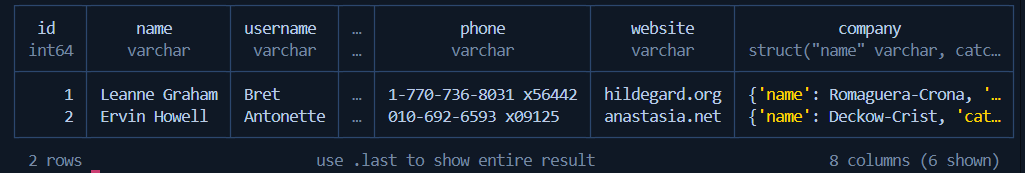
\includegraphics[width=0.9\textwidth]{imagenes/resultado_actividad1.png}
    \caption{Resultado de la consulta de la tabla con datos crudos.}
    \label{fig:resultado-actividad1}
\end{figure}
 
\subsection{Actividad 2: Consulta analítica de negocio}

Se elaboró un reporte consolidado por ciudad que muestra el total de usuarios,
el número de dominios de correo distintos y la extensión geográfica (latitud
mínima y máxima), restringido a ciudades que cuenten con al menos un usuario
cuyo \texttt{id} sea un número par.
 
La condición sobre el \texttt{id} par se aplicó con \texttt{HAVING} en lugar
de \texttt{WHERE}, ya que es una condición sobre el grupo (ciudad) y no sobre
cada fila individual; filtrar con \texttt{WHERE} antes de agrupar excluiría
usuarios de \texttt{id} impar del conteo total, alterando el resultado
solicitado.
 
\begin{lstlisting}[caption={Consulta analítica con funciones agregadas y extracción de subestructuras JSON}]
SELECT
    address.city AS ciudad,
    COUNT(id) AS total_usuarios,
    COUNT(DISTINCT regexp_extract(email, '@(.*)$', 1)) AS dominios_diferentes,
    MIN(CAST(address.geo.lat AS DOUBLE)) AS latitud_minima,
    MAX(CAST(address.geo.lat AS DOUBLE)) AS latitud_maxima
FROM datos_raw
GROUP BY address.city
HAVING SUM(CASE WHEN id % 2 = 0 THEN 1 ELSE 0 END) > 0
ORDER BY total_usuarios DESC, ciudad ASC;
\end{lstlisting}
 
% --- Aquí se inserta la captura del resultado de la consulta ---
\begin{figure}[h]
    \centering
    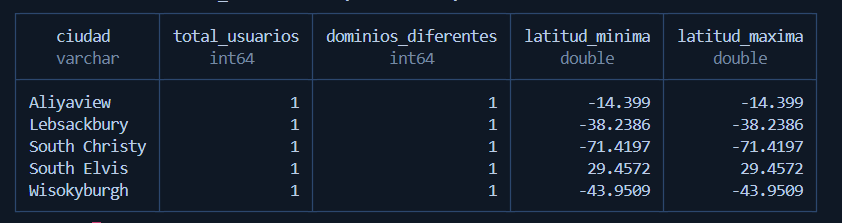
\includegraphics[width=0.9\textwidth]{imagenes/resultado_actividad2.png}
    \caption{Resultado de la consulta analítica por ciudad.}
    \label{fig:resultado-actividad2}
\end{figure}
 
\subsection{Actividad 3: Anonimización}
 
Se aplicaron los principios de \textit{Privacy by Design} y minimización de
datos. De los dos escenarios propuestos, se optó por el
\textbf{Escenario B (anonimización en la ingesta)}: se genera una vista
intermedia anonimizada inmediatamente después de leer la fuente primaria,
y la tabla persistente final solo conserva la versión anonimizada. La tabla
cruda (\texttt{datos\_raw}) se elimina una vez generada dicha vista, para
que la PII completa nunca quede disponible para consultas posteriores.
 
\begin{lstlisting}[caption={Anonimización mediante expresiones regulares (motor RE2) y limpieza de datos crudos}]
-- Escenario B: anonimizacion en la ingesta.
-- Se descarta la PII antes de que cualquier analista pueda consultarla,
-- cumpliendo Privacy by Design y minimizacion de datos.
 
CREATE VIEW v_datos_anonimizados AS
SELECT
    id,
    name,
    regexp_replace(email, '^(.{2}).*(@.*)$', '$1*****$2') AS email_protegido,
    regexp_replace(phone, '.*(.{4})$', '***-***-$1') AS telefono_protegido,
    address.city AS ciudad,
    company.name AS empresa
FROM datos_raw;
 
CREATE TABLE historico_usuarios_seguro AS
SELECT * FROM v_datos_anonimizados;

-- Visualizamos algunos datos de la tabla anonimizada:
SELECT * FROM historico_usuarios_seguro LIMIT 5; 

-- Eliminacion de la tabla cruda para no conservar PII en disco
DROP TABLE datos_raw;
\end{lstlisting}

% --- Aquí se inserta la captura del resultado de la consulta ---
\begin{figure}[h]
    \centering
    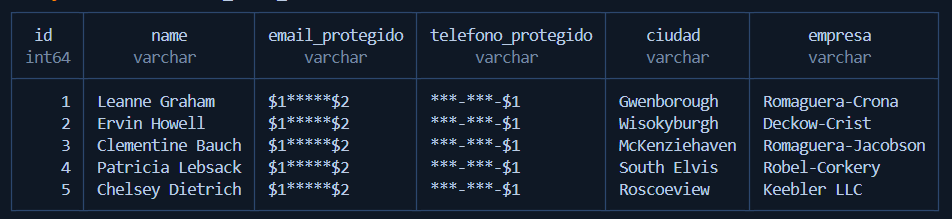
\includegraphics[width=0.9\textwidth]{imagenes/resultado_actividad3.png}
    \caption{Resultado de la consulta de la tabla con los datos seguros.}
    \label{fig:resultado-actividad3}
\end{figure}
 
\subsection{Registro de comandos (log)}
 
Para cumplir con el entregable del log de comandos, se redirigió la salida
del CLI de DuckDB hacia un archivo local antes de ejecutar la práctica, y se
restauró al finalizar.
 
\begin{lstlisting}[caption={Redirección de la salida del CLI a un archivo de log}]
-- 1. Redirigir la salida de la terminal a un archivo
.output log_comandos_numcontrol_U1.txt
 
-- 2. Activar el eco de los comandos ejecutados
.echo on
 
-- 3. A partir de aqui se ejecuta la practica normalmente
-- (Actividades 1, 2 y 3)
 
-- 4. Restaurar la salida a pantalla al finalizar
.output stdout
\end{lstlisting}
 
El archivo generado, \texttt{log\_comandos\_23680116\_U1.txt}, se adjunta
como entregable independiente en formato \texttt{.txt}.
 
% --- Aquí se puede insertar una captura del log generado ---
\begin{figure}[h]
    \centering
    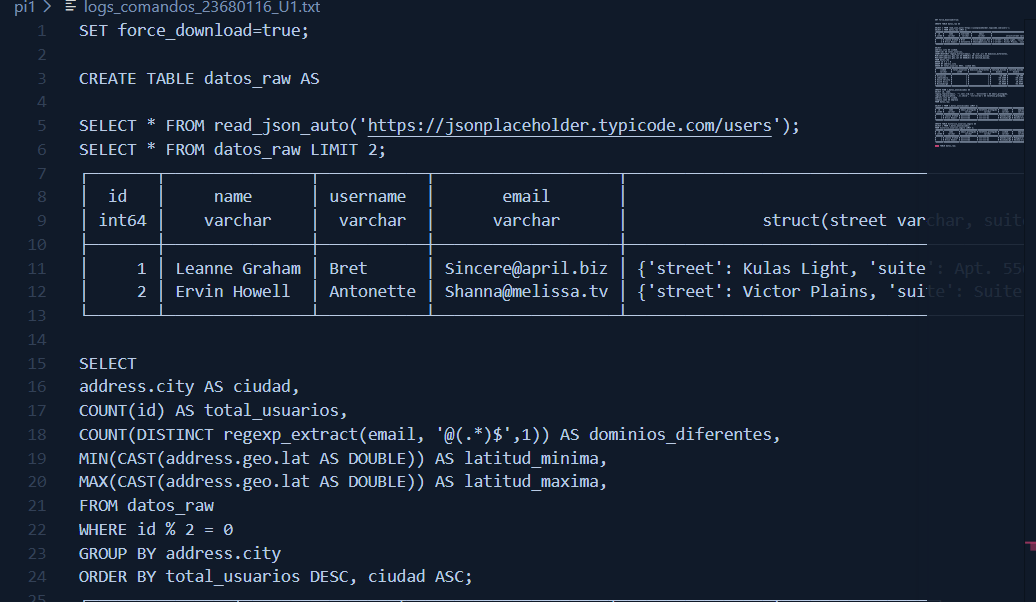
\includegraphics[width=0.9\textwidth]{imagenes/log-comandos.png}
    \caption{Fragmento del log de comandos generado por DuckDB CLI.}
    \label{fig:log-comandos}
\end{figure}
 

\section{Conclusión}
Este proyecto permitió poner en práctica, de manera integrada, los tres grandes temas de la unidad: cómo los datos apoyan la toma de decisiones, de dónde vienen y en qué forma llegan, y qué responsabilidad ética implica manejarlos. Más allá de las herramientas específicas utilizadas, el ejercicio deja una idea central: los datos por sí solos no dicen nada útil hasta que se organizan y resumen de forma que respondan una pregunta concreta, como en este caso conocer cuántos usuarios hay por ciudad o qué tan dispersos están geográficamente.

También quedó claro que trabajar con datos personales no es un detalle menor. Aunque la información utilizada era de prueba, el ejercicio de anonimizarla desde el primer momento ayuda a entender por qué la privacidad debe pensarse desde el diseño del sistema y no como un parche posterior. Esto conecta directamente con situaciones reales: cualquier proyecto que maneje información de personas, sin importar su tamaño, debería seguir este mismo criterio de proteger lo sensible desde el origen.

Finalmente, el proceso reforzó la importancia de documentar y dejar evidencia de cada paso realizado, no solo como requisito de entrega, sino como una buena práctica que facilita revisar, corregir y repetir el trabajo en el futuro si fuera necesario.


% =========================================================
% BIBLIOGRAFÍA
% =========================================================
\newpage

\bibliographystyle{ieeetr} % Estilo IEEE (puedes cambiarlo por apa, plain, etc.)
\bibliography{referencias} % Archivo .bib

\end{document}